\subsection{Actividades}

%%%%%%%%%%%%%%%%%%%%%%%%%%%%%%%%%%%%%%%%%%%%%%%%%%%%%%%%%%%%%%%%%%%%%%

\subsubsection[Revisión bibliográfica transformada de Hough.]{Revisión bibliográfica de aplicaciones de la transformada de Hough.}
<Tabla pendiente>

%%%%%%%%%%%%%%%%%%%%%%%%%%%%%%%%%%%%%%%%%%%%%%%%%%%%%%%%%%%%%%%%%%%%%%

\subsubsection[Código C de la T. Probabilística de Hough]{Implementación en C de la Transformada Probabilística de Hough.}

Bajo las mismas justificaciones por las que se decidió implementar en C la Transformada de Hough y, además, como resultado de los puntos expuestos en la revisión bibliográfica se decidió que se iba a desarrollar la Transformada Probabilística de Hough. Esta transformada no es matemáticamente una transformada porque, como dice su autor original en el paper donde la persentó, no se puede revertir.

\begin{figure}[ht!]
\begin{center}
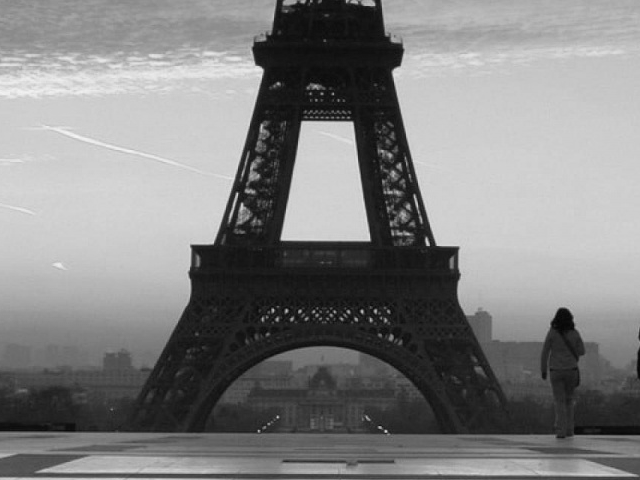
\includegraphics[height=0.4\textwidth]{fig/eiffel_grayscale}\\
\caption{Original Eiffel Tower grayscale image.}
\label{fig_eiffel_grayscale}
\end{center}
\end{figure}

\begin{figure}[ht!]
\begin{center}
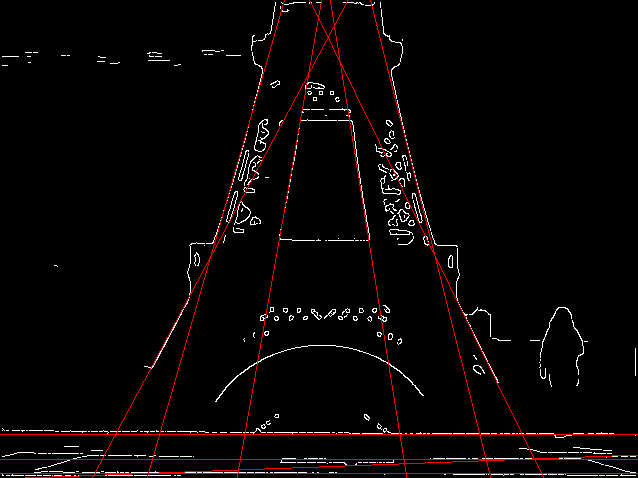
\includegraphics[height=0.4\textwidth]{fig/eiffel_hough}\\
\caption{Eiffel Tower image processed using the Hough Transform.}
\label{fig_eiffel_hough}
\end{center}
\end{figure}

\begin{figure}[ht!]
\begin{center}
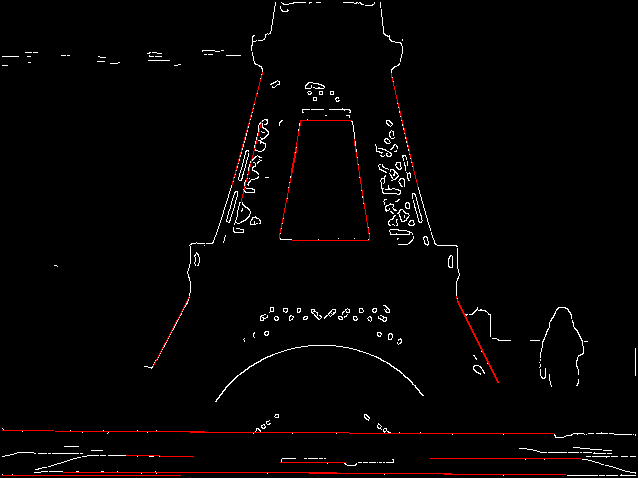
\includegraphics[height=0.4\textwidth]{fig/eiffel_phough}\\
\caption{Eiffel Tower image processed using the Probabilistic Hough Transform.}
\label{fig_eiffel_phough}
\end{center}
\end{figure}


\begin{itemize}
	\item Variante conceptual de la Transformada de Hough que resuelve (o atenúa) sus desventajas más importantes.
	\item OpenCV cuenta con la implementación de ambas: la Transformada de Hough y la Transformada Probabilística de Hough (más nueva y más usada).
\end{itemize}

\begin{table}
\begin{center}
\begin{tabular}{| l | c | c |}
\hline
\multicolumn{1}{|c|}{Parameter}	 & 	\multicolumn{1}{c|}{Traditional}	 & 	\multicolumn{1}{c|}{Probabilistic}\\ \hline
Total time (s)	& 	163.97	 &	154.52\\ \hline
Time per frame (ms)	& 	20.5	 & 	19.32\\ \hline
Frequency (Hz)		& 	48.79	 & 	51.77\\ \hline
\end{tabular}
\caption[Comparison of Hough transform algorithms.]{Comparison of Hough transform algorithms processing the same image 8000 times.}
\label{tab_compeiffel}
\end{center}
\end{table}


Con el objetivo de contextualizar se presenta una comparación del procesamiento sobre la misma imagen (Fig.~\ref{fig_eiffel_grayscale}) por ambos algoritmos para comparar los resultados. El resultado gráfico al utilizar el algoritmo tradicional se muestra en la figura \ref{fig_eiffel_hough}, mientras que la salida al utilizar la Transformada Probabilística se muetra en la figura \ref{fig_eiffel_phough}. La prueba consistió en procesar la imagen por ocho mil iteraciones, para evitar ruido de programas externos y ajenos al experimento. Los programas no se ejecutaron al mismo tiempo y había la misma cantidad de programas corriendo en la computadora cuando se hicieron las pruebas.

Se pueden hacer las siguientes observaciones en cuanto al nivel de similitud de los resultados:

\begin{itemize}
	\item En la versión tradicional no se está computando los puntos que delimitan la línea (por eso atraviesan toda la imagen).
	\item La versión probabilística detectó todas (y más) las líneas que detectó su contraparte.
	\item Comparando el tiempo que les tomó realizar la prueba se obtuvieron los resultados de la tabla \ref{tab_compeiffel}.
	\item El tiempo es despreciablemente menor para la Transformada Probabilística. Pero además esta transformada hace más cosas que la tradicional. Entonces hace más en menos tiempo.
	\item Los parámetros de búsqueda de líneas de la Transformada Tradicional estaban prácticamente "sintonizados'' y probados.
	\item Simplemente cambiando los parámetros de la Transformada Probabilística se pueden obtener mejores resultados (de por sí son buenos).
	\item Esto es, la transformada Tradicional se muestra funcionando al límite, mientras que la Probabilística todavía se puede mejorar.
\end{itemize}


%%%%%%%%%%%%%%%%%%%%%%%%%%%%%%%%%%%%%%%%%%%%%%%%%%%%%%%%%%%%%%%%%%%%%%

%\subsubsection{Exploración de proyectos de STM32.}


%%%%%%%%%%%%%%%%%%%%%%%%%%%%%%%%%%%%%%%%%%%%%%%%%%%%%%%%%%%%%%%%%%%%%%

\subsubsection{Planeación.}
La planeación del proyecto no se había hecho porque los objetivos no estaban bien definidos. Ahora que se definieron un poco mejor los objetivos era necesario separar el objetivo en tareas y esas tareas en subtareas para tener una percepción gráfica de la cantidad de tiempo requerirá el proyecto.

Se separó el objetivo en las siguientes secciones principales:
\begin{itemize}
	\item \textbf{STM32:} Código de adquisición y envío de imágenes.
	\item \textbf{Físico:} Hardware, montaje de cámaras en el vehículo, etcétera.
	\item \textbf{Raspberry:} Código de recepción de imágenes y gestión de tareas (prioridades, scheduler, etcétera).
	\item \textbf{Visión:} Procesamiento de imágenes.
	\item \textbf{Control:} Extracción de modelos, sintetización de control.
	\item \textbf{Paper:} Investigación necesaria, documentación y publicación de los resultados del proyecto.
\end{itemize}
